
\section{Wrapper}\label{sec:Wrapper}

\subsubsection*{Context} You are part of an active, long-running, and possibly quite complex project with more than a handful of participants.  

\subsubsection*{Problem} In an active project, it can be effectively impossible to stay up to date with all of the details.  Not everyone will be able to attend every meeting (see \patternname{Heartbeat}) or read every email.  Project participants can easily get lost and drift away.  The experience can be more difficult for \patternnameplural{Newcomer}: joining an existing project can feel like trying to get aboard a rapidly moving vehicle.  If you've taken time off, you may feel like things have moved on so far that you cannot catch up.  Information overload is not the only concern: there is also a problem with missing information.  If they aren't shared, key skills can quickly become bottlenecks (see \patternname{Carrying capacity}).

\subsubsection*{Solution}
% DK: Be more direct.  Don’t say what “can” be done…just say what to do. [also, typo -jc]
Someone involved with the project should regularly create a wrap-up summary, distinct from other project communications, that makes current activities comprehensible to people who may not have been following all of the details.  In addition, project members should keep other informative resources like the landing page, \patternname{Roadmap}, and documentation up to date.  Ensure that these resources accurately represent the facts on the ground, and check empirically to see if they really show interested parties how they can get involved.

\subsubsection*{Rationale}
According to the theory proposed by Yochai Benkler, for free/open ``commons-based'' projects to work, it is important for participants to the ability to contribute small pieces, and for the project to have a way to stitch those pieces together \cite{coases-penguin}.  The \patternname{Wrapper} helps perform this integrative stitching function.

\subsubsection*{Resolution} 
% DK: This sounds like Rationale
Regularly circulated summaries can help to engage or re-engage members of a project, and can give an emotional boost to peeragogues who see their contributions and concerns mentioned.  Well-maintained records chronicle the project's history; up-to-date documentation makes the project more accessible and robust.

\begin{framed}
\emph{What's Next.}
We have prototyped and deployed a visual ``dashboard'' that people can access to immediately get an idea of what work is ongoing in the project with links to ways to get further engaged (Figure \ref{dashboard}).  Let's improve it.
\end{framed}    


\begin{figure}
\begin{tikzpicture}[every node/.style={anchor=south west,inner sep=0pt},x=1mm, y=1mm,]
     \node (fig1) at (0,0)
       {\includegraphics[width=\textwidth,trim=0mm 135mm 0mm 0mm,clip=true]{figures/peeragogy_dashboard_draft1/peeragogy_dashboard_draft1.jpg}};
     \node (fig2) at (55, 14)
       {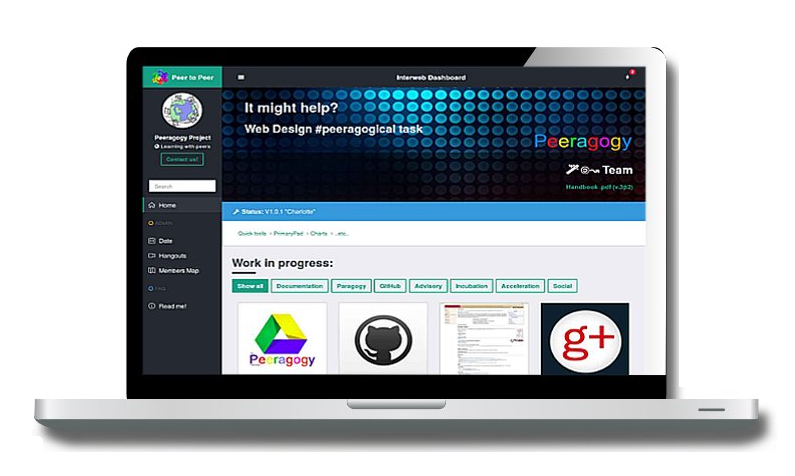
\includegraphics[width=.45\textwidth,trim=0mm 0mm 0mm 0mm,clip=true]{figures/dashboard/dash-trans.png}};  
\end{tikzpicture}
\caption{Design for a Peeragogy project dashboard (design sketch by Amanda Lyons, prototype by Fabrizio Terzi; images used with permission).\label{dashboard}}
\end{figure}

